% Drawing 154/08-29 -- folder 154, batch 08, archive page 156 (PDF page 157).
% Transcription: à droite, entre parenthèses au crayon, un dessin en couleur, source de la flèche $\rho_f$ : deux configurations réunies par « ou ». Dans chacune, une droite verte pleine coupe deux paires de droites orange, et une droite verte en tirets, au-dessus, passe par le premier croisement ; le triangle du premier croisement est marqué $T$, celui du second, hachuré au crayon, $T_1$ ; à gauche le second croisement est au-dessus des deux droites, à droite au-dessous ; de petites flèches au crayon opposées entre les deux triangles, avec le mot « lien » ; une flèche verte vers la droite
% Kind: in pencil brackets, two configurations joined by « ou »: solid green line, dashed line through the first crossing, triangles T and T_1 (source of rho_f). Method 2 (schematic redraw from the facsimile). Status: partial.
% Notes: In pencil brackets, where the arrow rho_f of the star diagram starts. Two configurations with « ou » between them. Left: a solid green line rising to the right crosses two pairs of orange lines below their crossings; green dashes above it go through the first crossing (the third dash ends in an arrowhead) and a longer dash crosses the second pair; T is written under the dashes left of the first pair; the triangle of the second pair, from its crossing down to the solid line, is hatched in pencil and marked T_1 (the transcription's reading of the mark, which looks like « T1 »); a small green arrow to the right beside T_1; under the solid line, between the pairs, two small pencil arrows pointing apart with the pencilled word « lien » between them (confirmed by the editor, #150: « Yes, as redrawn »). Right: the same with the second crossing below the solid line (a V), its small triangle between line and crossing hatched and marked T_1; the dashes go through the first crossing and over the second pair; two small pencil arrows pointing apart; a thick green arrow to the right. Left out: the pencilled legend of three short lines under the figure (read « prenons / lien de / triangles », « lien » confirmed, the other words uncertain) and the two curved strokes that join it to the pairs of small arrows; this is text for the transcription. 8 orange strokes, 4 crossings, 2 solid lines, 8 dashes, 3 green arrows, 4 pencil arrows. Read from the 400 dpi colour scan; each pair of orange strokes fitted to the ink and drawn through its computed crossing, the triangles bounded by the computed intersections with the green line; the redraw was overlaid on the scan and agrees to within a stroke's width. The felt strokes are drawn straight (slight curvature of a few strokes not reproduced). Redrawn 2026-11-12 (issue 128): to check again.
% Coordinates: 1 unit = 1 mm = 1/100 of the crop width, same scale on both axes (bbox in page fractions: [0.597, 0.165, 0.933, 0.222]).
% Redrawn by Claude (claude-fable-5-2), issue #128, 2026-11-12; not checked by a human; not compiled (no TeX in the session).
% Rights: reproduces part of the work -- behind RENDER_TRANSCRIPTS, never published by itself.
\documentclass[tikz,border=3pt]{standalone}
\usepackage{amsmath,amssymb}
\usetikzlibrary{patterns,arrows.meta}
\tikzset{Or/.style={orange!90!black}, Lg/.style={green!60!black!70}, Br/.style={brown!80!black}, pencil/.style={black!55}, mpt/.style={circle,draw,inner sep=1.3pt}, pt/.style={circle,fill,inner sep=0.9pt}}
\colorlet{Or}{orange!90!black}\colorlet{Lg}{green!60!black!70}\colorlet{Br}{brown!80!black}
\begin{document}
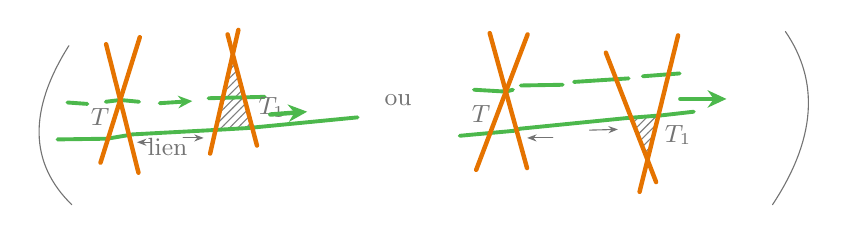
\begin{tikzpicture}[x=1mm,y=1mm,line cap=round,line join=round,font=\scriptsize]
\path[pattern=north east lines,pattern color=black!50] (25.41,-4.32) -- (23.22,-13.94) -- (27.88,-13.65) -- cycle;
\path[pattern=north east lines,pattern color=black!50] (78.08,-17.73) -- (79.46,-12.11) -- (76,-12.39) -- cycle;
\draw[pencil] (4.59,-3.24) .. controls (-0.57,-11.41) and (-0.45,-18.14) .. (4.95,-23.42);
\draw[pencil] (95.59,-1.44) .. controls (99.97,-7.81) and (99.43,-15.14) .. (93.96,-23.42);
\draw[Lg,line width=1.4pt] (3.15,-15.14) -- (9.46,-15.05) -- (12.7,-14.5) -- (22.79,-13.96) -- (27.39,-13.69) -- (41.26,-12.34);
\draw[Lg,line width=1.4pt] (4.41,-10.45) -- (6.94,-10.63);
\draw[Lg,line width=1.4pt] (9.28,-10.36) -- (11.11,-10.13) -- (13.51,-10.36);
\draw[Lg,line width=1.4pt,-{Stealth[length=1.8mm,width=1.6mm]}] (16.13,-10.54) -- (20.27,-10.27);
\draw[Lg,line width=1.4pt] (22.34,-9.91) -- (29.46,-9.73);
\draw[Or,line width=1.6pt] (9.32,-3.05) -- (11.11,-10.13) -- (13.43,-19.37);
\draw[Or,line width=1.6pt] (13.6,-2.16) -- (11.11,-10.13) -- (8.61,-18.09);
\draw[Or,line width=1.6pt] (26.12,-1.23) -- (25.41,-4.32) -- (22.53,-16.94);
\draw[Or,line width=1.6pt] (24.75,-1.8) -- (25.41,-4.32) -- (28.48,-15.92);
\node[pencil,inner sep=1pt] at (8.56,-12.25) {\small $T$};
\node[pencil,inner sep=1pt] at (30.36,-11.08) {\small $T_1$};
\draw[pencil,-{Stealth[length=1.2mm]}] (15.05,-15.5) -- (13.24,-15.5);
\draw[pencil,-{Stealth[length=1.2mm]}] (19.1,-14.95) -- (21.71,-14.95);
\node[pencil,inner sep=1pt] at (17.12,-16.04) {\small lien};
\draw[Lg,line width=1.6pt,-{Stealth[length=2.4mm,width=2.2mm]}] (30.18,-11.98) -- (34.86,-11.62);
\node[pencil,inner sep=1pt] at (46.4,-10.09) {\small ou};
\draw[Lg,line width=1.4pt] (54.23,-14.68) -- (61.08,-14.05) -- (61.89,-13.78) -- (75.41,-12.43) -- (80,-12.07) -- (83.96,-11.62);
\draw[Lg,line width=1.4pt] (56.04,-8.83) -- (60.09,-9.07) -- (60.99,-8.83);
\draw[Lg,line width=1.4pt] (61.98,-8.29) -- (67.3,-8.2);
\draw[Lg,line width=1.4pt] (68.74,-7.84) -- (75.68,-7.39);
\draw[Lg,line width=1.4pt] (77.48,-7.12) -- (82.16,-6.76);
\draw[Or,line width=1.6pt] (58.04,-1.64) -- (60.09,-9.07) -- (62.78,-18.78);
\draw[Or,line width=1.6pt] (62.85,-1.81) -- (60.09,-9.07) -- (56.32,-19.01);
\draw[Or,line width=1.6pt] (81.96,-1.93) -- (78.08,-17.73) -- (77.07,-21.8);
\draw[Or,line width=1.6pt] (72.79,-4.13) -- (78.08,-17.73) -- (79.17,-20.55);
\node[pencil,inner sep=1pt] at (56.94,-11.89) {\small $T$};
\node[pencil,inner sep=1pt] at (81.98,-14.59) {\small $T_1$};
\draw[pencil,-{Stealth[length=1.2mm]}] (66.04,-14.95) -- (62.79,-14.95);
\draw[pencil,-{Stealth[length=1.2mm]}] (70.72,-13.96) -- (74.32,-13.87);
\draw[Lg,line width=1.6pt,-{Stealth[length=2.4mm,width=2.2mm]}] (82.25,-10) -- (88.11,-10);
\end{tikzpicture}
\end{document}
